\hypertarget{sh__find_8c}{
\section{sh\_\-find.c File Reference}
\label{sh__find_8c}\index{sh_find.c@{sh\_\-find.c}}
}


\subsection{Detailed Description}
\begin{Desc}
\item[For internal use only.]
This file contains the implementation of the \hyperlink{group__dbprim__smat_ga20}{sh\_\-find()} function, used to look up a specific \hyperlink{group__dbprim__smat_ga2}{smat\_\-entry\_\-t} in a sparse matrix head.\end{Desc}


Definition in file \hyperlink{sh__find_8c-source}{sh\_\-find.c}.

{\tt \#include \char`\"{}dbprim.h\char`\"{}}\par
{\tt \#include \char`\"{}dbprim\_\-int.h\char`\"{}}\par


Include dependency graph for sh\_\-find.c:\begin{figure}[H]
\begin{center}
\leavevmode
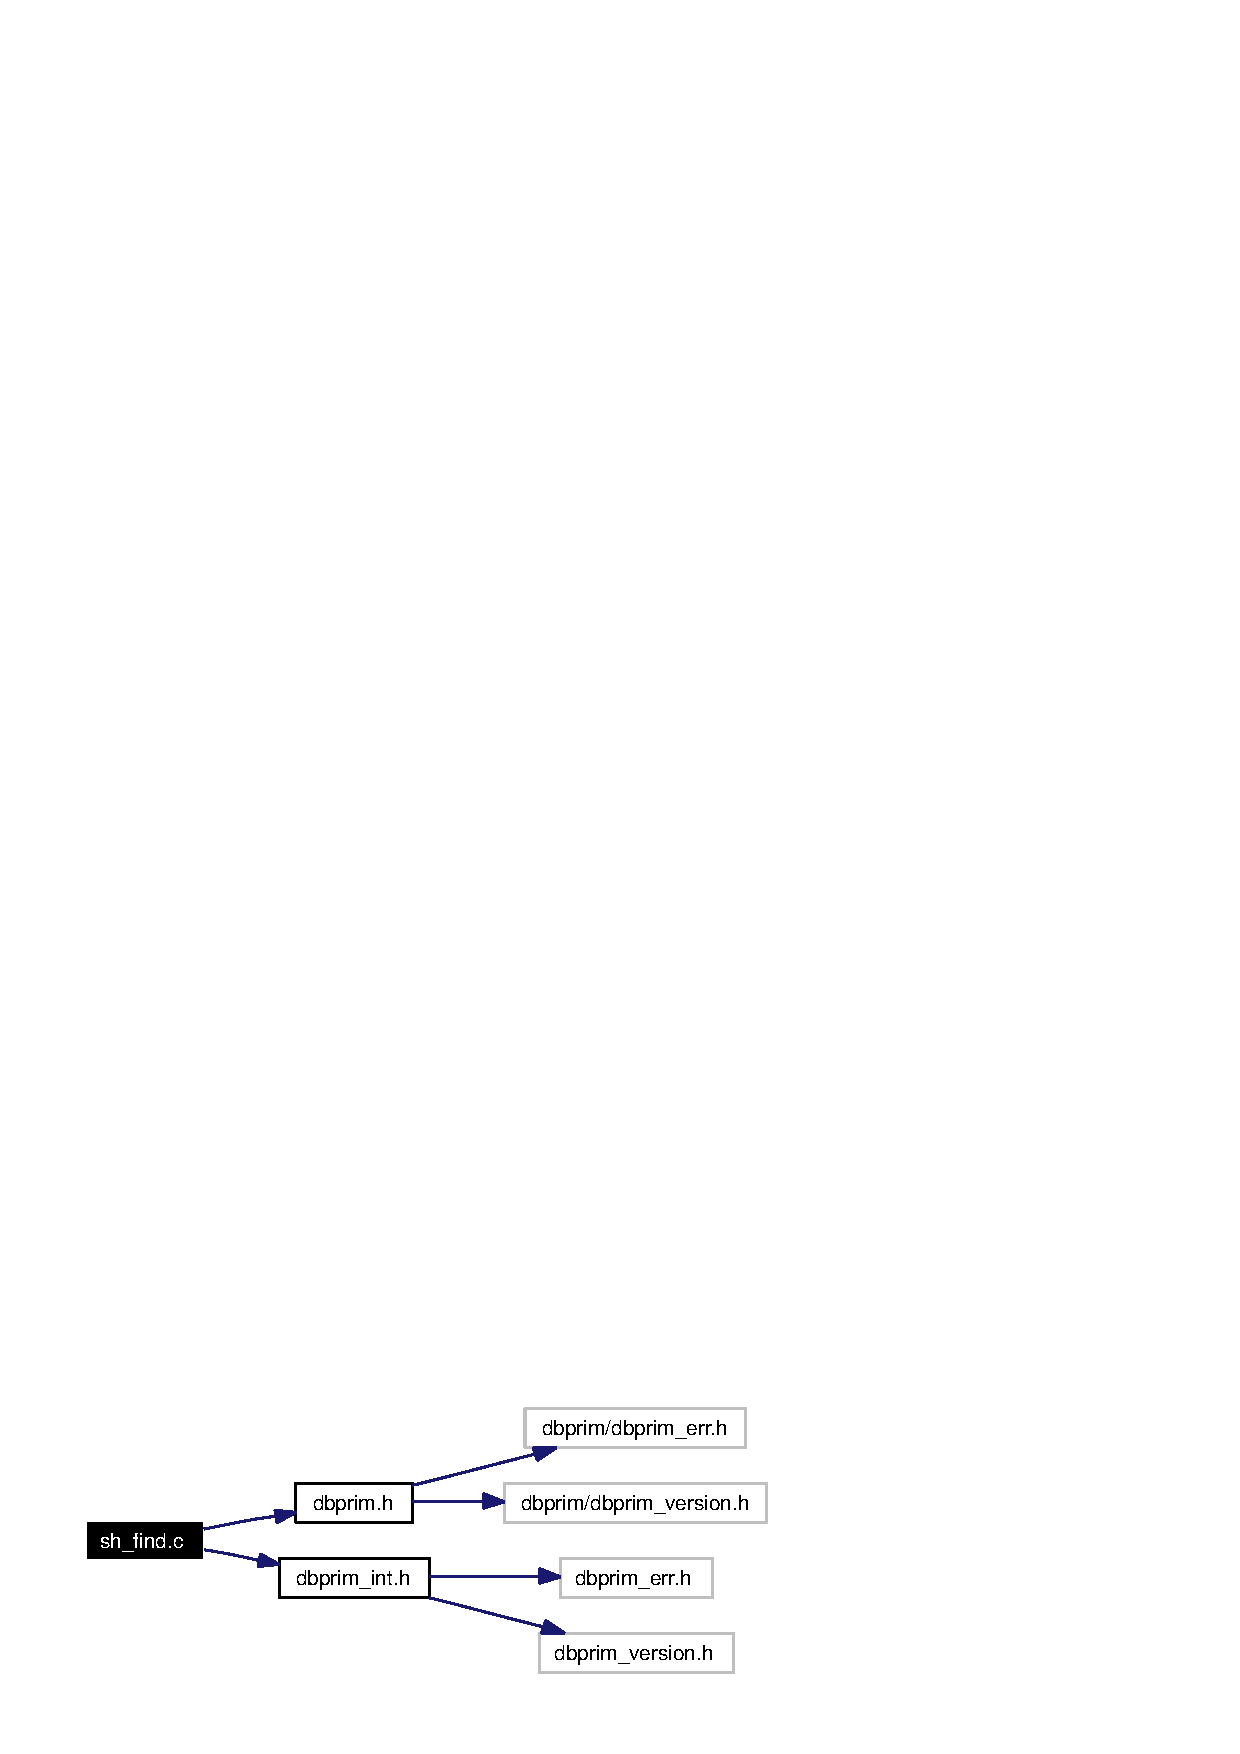
\includegraphics[width=186pt]{sh__find_8c__incl}
\end{center}
\end{figure}
\subsection*{Data Structures}
\begin{CompactItemize}
\item 
struct \hyperlink{struct__sh__find__s}{\_\-sh\_\-find\_\-s}
\begin{CompactList}\small\item\em Sparse matrix head find shim structure. \item\end{CompactList}\end{CompactItemize}
\subsection*{Functions}
\begin{CompactItemize}
\item 
static unsigned long \hyperlink{group__dbprim__smat_ga27}{\_\-sh\_\-find\_\-comp} (\hyperlink{struct__db__key__s}{db\_\-key\_\-t} $\ast$key, void $\ast$data)
\begin{CompactList}\small\item\em Sparse matrix linked list comparision function. \item\end{CompactList}\item 
unsigned long \hyperlink{group__dbprim__smat_ga20}{sh\_\-find} (\hyperlink{struct__smat__head__s}{smat\_\-head\_\-t} $\ast$head, \hyperlink{struct__smat__entry__s}{smat\_\-entry\_\-t} $\ast$$\ast$elem\_\-p, \hyperlink{group__dbprim__smat_ga5}{smat\_\-comp\_\-t} comp\_\-func, \hyperlink{struct__smat__entry__s}{smat\_\-entry\_\-t} $\ast$start, \hyperlink{struct__db__key__s}{db\_\-key\_\-t} $\ast$key)
\begin{CompactList}\small\item\em Find an entry in a row or column of a sparse matrix. \item\end{CompactList}\end{CompactItemize}
